%==============================================================================
% Sjabloon onderzoeksvoorstel bachproef
%==============================================================================
% Gebaseerd op document class `hogent-article'
% zie <https://github.com/HoGentTIN/latex-hogent-article>

% Voor een voorstel in het Engels: voeg de documentclass-optie [english] toe.
% Let op: kan enkel na toestemming van de bachelorproefcoördinator!
\documentclass{hogent-article}

% Invoegen bibliografiebestand
\addbibresource{voorstel.bib}

% Informatie over de opleiding, het vak en soort opdracht
\studyprogramme{Professionele bachelor toegepaste informatica}
\course{Bachelorproef}
\assignmenttype{Onderzoeksvoorstel}
% Voor een voorstel in het Engels, haal de volgende 3 regels uit commentaar
% \studyprogramme{Bachelor of applied information technology}
% \course{Bachelor thesis}
% \assignmenttype{Research proposal}

\academicyear{2023 - 2024} 

\title{Gitlab vs Jenkins pipeline: een vergelijkende studie over het hosten van Python scripts op de IBM Z Systems}

\author{Alif Monnoye}
\email{alif.monnoye@student.hogent.be}

% TODO: Geef de co-promotor op
\supervisor[Co-promotor]{ Njaal Sletten, \email{njaal.sverre.slette@dnb.no} } %J. Doe (X, \href{mailto:sigrid.beekman@synalco.be}{sigrid.beekman@synalco.be})}


\specialisation{Mainframe Expert}
\keywords{Python scripts, Mainframe, Gitlab Pipeline, Jenkins, CI/CD}

\begin{document}

\begin{abstract}
  De IBM Z Systems hebben nood aan een opfrissing in technieken zonder zijn bruikbaarheid en kracht te verliezen. Python is één van de meest gebruikte programmeertalen ter wereld met veel functionaliteiten wat perfect is voor te draaien op de mainframe. Niet alleen voor zijn kracht en functionaliteit, maar ook voor zijn bekendheid onder programmeurs. Deze scripts worden door een Continuous integration/continuous deployment (CI/CD) automatisch ingezet om gebruikt te worden op de mainframe. Hierdoor is dit makkelijker voor een DevOps teams zonder geavanceerde mainframe kennis om scripts te schrijven voor deze omgeving.   \\
  Deze paper zal twee verschillende CI/CD pipelines vergelijken namelijk Gitlab Pipeline en Jenkins. Er zal gekeken worden naar de gelijkenissen en verschillen voor het opstellen van deze technieken. Ook zal er bestudeerd hoe deze pipelines werken om de python scripts uit te voeren. Zo kunnen we evalueren welke het efficiëntst is voor welk soort project of opdracht.
\end{abstract}

\tableofcontents

% De hoofdtekst van het voorstel zit in een apart bestand, zodat het makkelijk
% kan opgenomen worden in de bijlagen van de bachelorproef zelf.
%---------- Inleiding ---------------------------------------------------------
\newpage
\section{Introductie}%
\label{sec:introductie}
In de huidige technologische wereld is het moeilijk bij te houden welke mogelijkheden er zijn om bepaalde projecten uit te voeren. Zo heb je altijd nieuwe technieken die net iets efficiënter of krachtiger zijn dan een ander. Door deze voortgaande evolutie zullen individuen niet direct op de hoogte zijn van recente ontwikkelingen, maar vergeten ze ook de oudere toepassingen van een bepaalde techniek. Dit is vooral merkbaar bij IBM hun z Systems of mainframes die zo belangrijk, maar zo snel vergeten worden in de IT wereld. Hoewel het een zeer hoogwaardige technologie is, zijn de technieken nog steeds zeer oud. Hier wordt wel op ingezet door modernere talen zoals Java en Python compatibel te maken met dit systeem. Een veel gebruikte tool, aangeboden door IBM, is IBM Developer for z/OS. Dit is een Eclipse based programma geschreven in Java en kan een connectie maken met de mainframe en zijn opgeslagen bestanden. Dit maakt het eenvoudiger voor gebruikers om verschillende bestanden te openen maar heeft geen Python interpreter waardoor het voor developers niet zo efficiënt is om Python programma's aan te passen.


\subsection{Probleemstelling}
Het bedrijf waar het onderzoek in wordt uitgevoerd is Den Norske Bank (DNB) met een hoofdvestiging in Oslo, Noorwegen. Hun developers zoals Stian Botnevik zitten vast met het beschreven probleem en zoeken een efficiëntere manier om Python scripts te schrijven en testen. Momenteel passen ze Python scripts aan in een text editor van IBM Developer for z/OS (IDz) en testen ze de code in een ssh connectie. \\
Python scripts worden opgeslagen en uitgevoerd in de Unix System Services (USS) omgeving. Dit is een Unix omgeving op de mainframe. In IDz kunnen developers alle bestanden openen in de USS omgeving wat duidelijker is dan code aanpassen in een terminal via bijvoorbeeld de vim tool.  


%---------- Stand van zaken ---------------------------------------------------

\section{State-of-the-art}%
\label{sec:state-of-the-art}

\subsection{Een andere manier van werken}
Veel bedrijven die werken met een mainframe hebben het probleem dat ze onvoldoende mensen vinden met de nodige kennis over deze technologie. De introductie van Unix systemen op de mainframe in het jaar 2000 \autocite{Mertic2020} had dit probleem wat verminderd maar zeker niet weggewerkt. De oorzaak van deze situatie is door de oude technieken die het systeem gebruikt. COBOL en PL/1 zijn niet de meest aantrekkelijke programmeertalen om te leren en mensen kiezen liever Bash als scripttaal in plaats van REXX. Hoewel IBM veel inzet op documentatie en online leerplatformen zoals IBM Z Xplore, blijft het tekort van ervaren mensen nog steeds te laag. \\

De mainframe wereld zal zich dus moeten aanpassen aan de vaardigheden van de mensen door over te schakelen naar bekendere manieren van werken. 
Python bijvoorbeeld is een programmeertaal die steeds meer populariteit krijgt sinds zijn creatie in de vroege jaren 90 \autocite{Johnson2023}. Dit is niet enkel bij reeds ervaren programmeurs, maar mensen die net beginnen programmeren kiezen hier steeds vaker voor. Dit is vooral door zijn begin vriendelijkheid, verschillende doeleinden en een actieve community. \autocite{Johnson2023} \\

IBM heeft dit opgemerkt en een Python compiler en interpreter ontwikkeld voor z/OS genaamd IBM Open Enterprise SDK for Python. Hierdoor kun je met Python interactie hebben met z/OS om bijvoorbeeld applicaties te ontwikkelen of de resources van het systeem te gaan beheren. Door de Unix omgeving heeft de programmeur ook geen speciale z/OS kennis nodig. \autocite{Klaey2023} \\

\subsection{Bedrijven in het werkveld}
Een bank is een goed voorbeeld van een bedrijf die gebruik maakt van IBM hun mainframes. Dit valt te concluderen door het feit dat maar liefst 92 van de top 100 banken wereldwijd een mainframe gebruikt. Dit is ook logisch aangezien er gemiddeld 12.6 miljard financiële transacties per dag uitgevoerd worden. \autocite{Wagle2017} \\

Door dit aantal is de nood voor een mainframe toch niet te onderdrukken maar het is niet enkel het aantal transacties dat deze machine kan uitvoeren, het is ook de snelheid, schaalbaarheid en beveiliging van deze systemen dat een grote rol speelt. Het zijn ook niet enkel banken die van deze technologie gebruik maken, maar ook  verzekeringsmaatschappijen bijvoorbeeld. De top 10 van deze soort bedrijven maken allemaal gebruik van een IBM mainframe. \autocite{Tozzi2022}

\subsection{De Skill gap}
Het is nog steeds moeilijk om nieuw talent aan te trekken in de mainframe wereld. Een onderzoek van \textcite{Deloitte2020} toont aan dat 79\% van de projectleiders moeilijkheden heeft met het zoeken naar mensen met de juiste skillset. Hetzelfde onderzoek toont ook aan dat er in de teams zelf een groot verschil is van kennis en vaardigheden. Hoewel dit systeem gebruikt wordt door 71\% van de fortune 500 companies \autocite{Tozzi2022} , is de Skill gap nog steeds te groot waardoor veel bedrijven vrezen voor een groot tekort aan werknemers om deze z Systems te onderhouden. \\

Volgens Petra \textcite{Goude2023} zijn er verschillende manieren om dit probleem aan te pakken. Zo kunnen bedrijven lessen geven over mainframes en hoe ze dit gebruiken. Ze vertelt ook dat de vaardigheden die nodig zijn beter gecomplimenteerd moeten worden en kunnen leiden naar een belonende en lange termijn carrière. \\ 

Hoewel dit zou helpen, vind ze dit niet de kern van het probleem. Het zijn de oude technieken die mensen niet aantrekt. Ze stelt voor om meer te investeren in hedendaagse technologie en dit te installeren op de mainframe. Dit kan gaan over dezelfde test -en deployment technieken, maar ook over hedendaagse programmeertalen zoals Java of Python. Dit zou kunnen door middel van APIs en zou een nieuwe, jongere werkkracht aantrekken. \autocite{Goude2023}


\subsection{Toch nog een kleurrijke toekomst}
Ondanks de grote nood aan mensen met de juiste vaardigheden, ziet de toekomst er toch nog goed uit. Zo wordt er meer gemoderniseerd met bijvoorbeeld modernere programmeertalen. Er wordt ook voorspeld dat we een introductie van DevOps en self-service benaderingen gaan zien. \autocite{Pennaz2023} \\

Momenteel zijn Python en Java beschikbaar als programmeertaal op de mainframe naast PL/1 en COBOL.
Sinds deze introductie zijn al bijna 2/3de van gebruikers op de mainframe Java aan het toepassen op een bepaalde manier. \autocite{Watts2018}

% Voor literatuurverwijzingen zijn er twee belangrijke commando's:
% \autocite{KEY} => (Auteur, jaartal) Gebruik dit als de naam van de auteur
%   geen onderdeel is van de zin.
% \textcite{KEY} => Auteur (jaartal)  Gebruik dit als de auteursnaam wel een
%   functie heeft in de zin (bv. ``Uit onderzoek door Doll & Hill (1954) bleek
%   ...'')


%---------- Methodologie ------------------------------------------------------

\section{Methodologie}%
\label{sec:methodologie}
Deze paper zal als resultaat een volledig stappenplan geven om Pydev op te stellen in IDz en verdere configuratie om de scripts uit te voeren in IDz.

\subsection{Fase 1: Literatuurstudie}
\begin{itemize}
    \item \textbf{Doel:}
    Relevante informatie verzamelen van IDz, Pydev en de Unix System Services omgeving.
    \item \textbf{Aanpak:}
    \item[-] Opzoeken betrouwbare bronnen
    \item[-] Gelijke projecten onderzoeken
    \item[-] Overzicht van nodige software
    \item \textbf{Tijd:} 5 weken
    \item \textbf{Opbrengst:}
    Een volledig onderzoek naar vakliteratuur en nodige software die nodig is. Ook een volledige schets naar de omgeving waarin er wordt gewerkt.
\end{itemize}


\subsection{Fase 2: Opstellen Pydev}
\begin{itemize}
    \item \textbf{Doel:}
    Opzetten van de Pydev plug-in in IDz
    \item \textbf{Aanpak:}
    \item[-] De opgezochte literatuur bestuderen
    \item[-] Pydev opstellen met de juiste vereisten
    \item[-] Testen
    \item \textbf{Tijd:} 3 weken
    \item \textbf{Opbrengst:}
    Pydev voor functies zoals code completion, syntax check, code analysis, ... \\ 
    Bij het openen van een Python programma zal dit ook gebeuren via een Python editor
\end{itemize}


\subsection{Fase 3: Python interpreter opzetten}
\begin{itemize}
    \item \textbf{Doel:}
    Python Interpreter opstellen om Python programma's uit te voeren in IDz.
    \item \textbf{Aanpak:}
    \item[-] De opgezochte literatuur bestuderen met expert
    \item[-] Opzetten van de juiste interpreter
    \item[-] Testen
    
    \item \textbf{Tijd:} 2 weken
    \item \textbf{Opbrengst:}
    Python programma's kunnen uitvoeren in IDz.
\end{itemize}


\subsection{Fase 4: Verdere configuratie om de output van de mainframe in de IDz console te krijgen}
\begin{itemize}
    \item \textbf{Doel:}
    Onderzoeken welke functies er beschikbaar zijn in Pydev
    \item \textbf{Aanpak:}
    \item[-] Pydev documentatie bekijken
    \item[-] Zelf onderzoeken in IDz
    
    \item \textbf{Tijd:} 2 weken
    \item \textbf{Opbrengst:}
    Een overzicht van alle functies die beschikbaar zijn. 
\end{itemize}

\subsection{Fase 5: Evaluatie voorbereiding}
\begin{itemize}
    \item \textbf{Doel:}
    Eind evaluatie voorbereiden
    \item \textbf{Aanpak:}
    \item[-] Resultaat bespreken, vergelijken en concluderen
    \item[-] Op orde stellen van nodige documenten
    \item \textbf{Tijd:} 2 weken
    \item \textbf{Opbrengst:}
    Een eind evaluatie waarin de opdracht besproken wordt
\end{itemize}


%---------- Verwachte resultaten ----------------------------------------------
\section{Verwacht resultaat, conclusie}%
\label{sec:verwachte_resultaten}
Een volledig stappenplan voor de opstelling van Pydev en een Python interpreter die compatibel is met IDz. Ook zal de configuratie getoond worden om de output van Python programma's te zien in IDz. Hierbij zal er bij elke stap uitleg gegeven worden over waarom het op die bepaalde manier gedaan wordt. Ook zal er besproken worden wat er mogelijks mis zou kunnen gaan. Screenshots zullen gebruikt worden voor duidelijk te maken wat er gebeurd. \\ 

Door de Pydev plug-in zal de interpreter eenvoudig opgesteld kunnen worden. Hier worden wel wat problemen verwacht omdat Pydev voor standaard Eclipse is ontwikkeld en IDz is hier een afstamming van waardoor er bepaalde onderdelen anders kunnen zijn. 


 

\printbibliography[heading=bibintoc]

\cleardoublepage
%\usepackage{graphicx}
\begin{figure}[pt!]
    \centering
    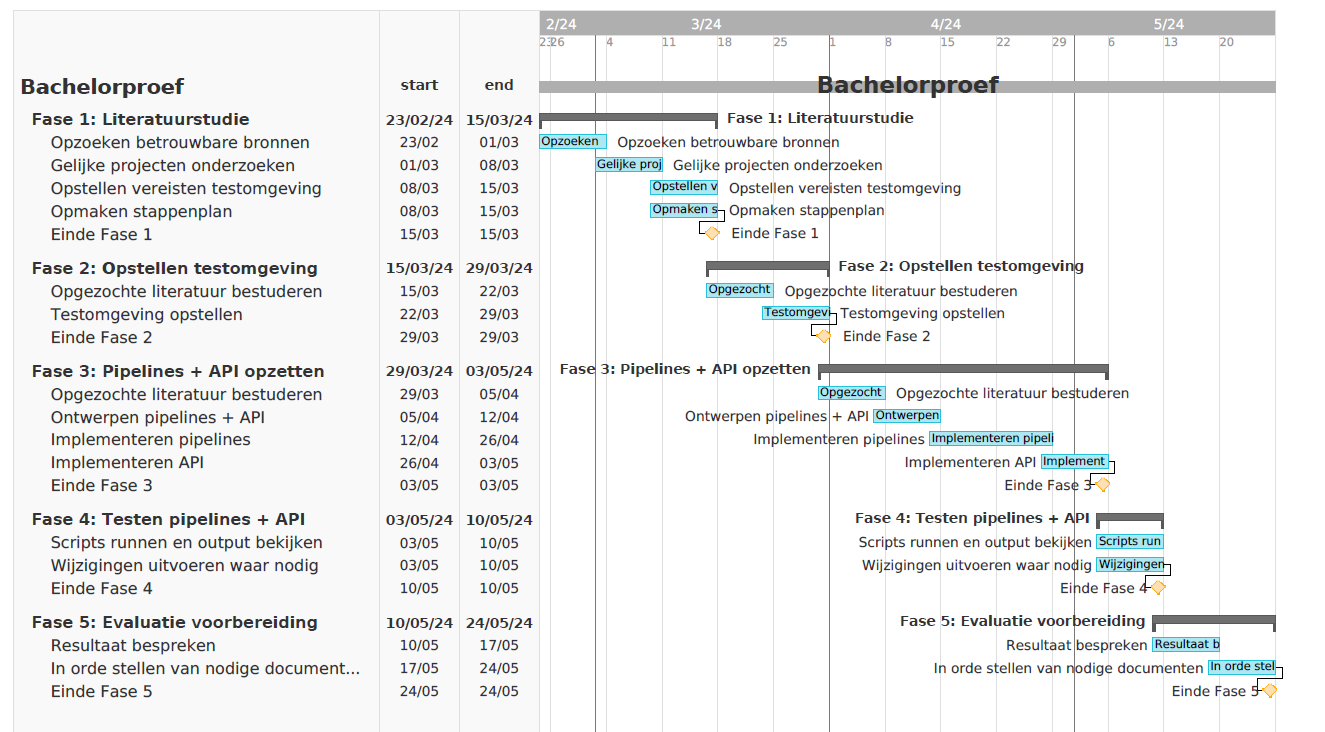
\includegraphics[width=550pt]{GanttChart.png}
    \caption{Gantt Chart}
    \label{fig}
\end{figure}


\end{document}